%!TEX root = ../template.tex
%%%%%%%%%%%%%%%%%%%%%%%%%%%%%%%%%%%%%%%%%%%%%%%%%%%%%%%%%%%%%%%%%%%%
%% chapter4.tex
%% NOVA thesis document file
%%%%%%%%%%%%%%%%%%%%%%%%%%%%%%%%%%%%%%%%%%%%%%%%%%%%%%%%%%%%%%%%%%%%

\typeout{NT FILE chapter4.tex}%

\chapter{Solution}
\label{cha:solution}

\prependtographicspath{{Chapters/Figures/Covers/}}

\glsresetall
 
\section{Threat Modeling Protocol for Horizontal Organizations}
\label{sec:protocol}

\subsection{Key Design Principles}
\label{subsec:key_principles}

\begin{itemize}
    \item \textbf{Transparency}: Security activities like decisions,
configurations and incidents should be visible to members. Open logs and
auditable records ensure nothing happens behind closed doors, building trust
and accountability among the group.
    \item \textbf{Decentralization}: No single person should have unchecked
power over systems or data. Access and control are distributed. This prevents a
single admin from being a weak link and avoids creating a digital vanguard
where a tech savvy few hold all the keys.
    \item \textbf{Democratic Participation}: All members can participate in
identifying and addressing threats. Security decisions are made through
inclusive discussions or votes, so measures are collective. This keeps
the process aligned with the cooperative's democratic governance.
    \item \textbf{Traceability}: Every important action like granting access or making
a change leaves an immutable trail. For example, changes can be logged on
tamper proof ledgers and digitally signed by those who approved them. This way,
if something goes wrong, the cooperative can trace what happened and who was involved,
without relying on memory or hearsay.
    \item \textbf{Resilience}: The protocol aims to strengthen the cooperative's
ability to withstand and recover from threats. By eliminating single failure
points and planning for crises with backup plans and rapid response
mechanisms, the organization stays resilient even under attack.
\end{itemize}

These principles ensure that improving security will not undermine the
organization nature of the group. Instead, security measures will reinforce
collaboration, shared responsibility, and trust. What
follows is a step by step threat modeling process designed with these values in
mind. Each step includes guidance and checklists for participatory activities,
and the protocol can be scaled or adapted for organizations of different
sizes and structures.

While this protocol is inspired by established frameworks like PASTA,
it does not use the formal seven stage PASTA terminology. Instead, it
presents an equivalent logic in a more accessible format focusing on
horizontal scenarios.

\subsection{Target Audience}
\label{subsec:target_audience}

The protocol is designed for members of horizontal organizations without
specialized cybersecurity expertise. Unlike traditional expert oriented models,
our protocol emphasizes simplicity and accessibility. It supports members
involved in decision making, operational activities, conflict resolution, and
coordination tasks, as well as informal community groups, by providing clear
guidance and intuitive methods for effectively dealing with security threats.

\section{Threat Modeling Process Overview}
\label{sec:threat_modeling_process_overview}

The threat modeling process is broken into eight collaborative steps. In a small
cooperative, most steps can be taken in all hands meetings or workshops with
everyone. In larger groups, you might delegate initial work to
working groups, but every member should have a chance to review and contribute
at each stage. The process is iterative and modular, so you can adjust the depth
or format of each step based on your organization's size and needs. For each
step below we describe the process and its activities.

\begin{figure}[htbp]
    \centering
    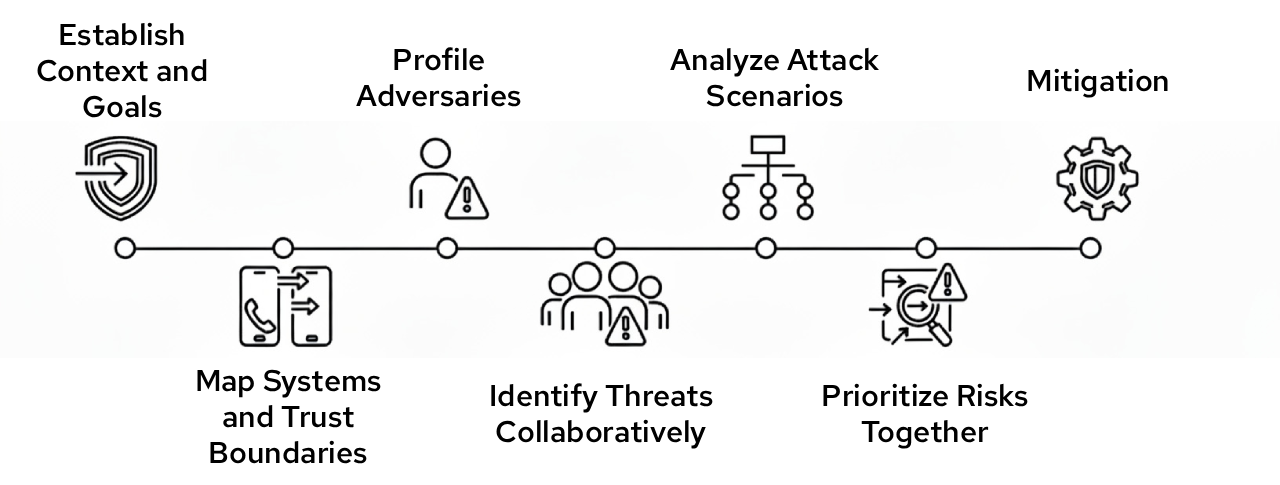
\includegraphics[width=1\linewidth]{protocol.png}
    \caption{Process overview.}
    \label{fig:process_overview}
\end{figure}

\subsection{Step 1: Establish Context and Goals}
\label{subsec:Step1}

What Are We Protecting?

\subsubsection{Purpose}

Set the stage by agreeing on what assets and operations you need to protect, and
what your security objectives are. This ensures everyone is on the same page
about why you are doing threat modeling and what success looks like. 

\subsubsection{Activities}

\begin{itemize}
    \item \textbf{Identify Critical Assets}: In a group, list out what is most
valuable to your organization. This can include digital assets as member data,
documents, the website, chat platforms or physical assets as office space, devices,
servers or intangible assets as the organization's reputation, member trust.
Ask yourselves what would hurt the most if it were stolen, destroyed, or made
public.
    \item \textbf{Outline Key Operations/Workflows}: Describe in simple terms
what the organization does everyday. For example, "We coordinate orders through an
online platform", or "We have weekly meetings to make decisions", or "We run a
community space with an entry badge system". Understanding these workflows helps
identify where disruptions would be most damaging.
    \item \textbf{State Security Objectives and Requirements}: Discuss what
security means for your organization. Do you need to keep member data private? Ensure
your service is always available? Meet any legal regulations like GDPR? Also consider
organization statutes or policies about confidentiality and data handling.
For instance, if your statutes say all financial info must be accessible
to members, that influences how you balance transparency with confidentiality.
    \item \textbf{Define the Scope and Boundaries}: Decide what will and won't
be covered in this threat modeling exercise. Maybe you want to focus on a
particular system and not on unrelated areas. Or include only digital systems but not
physical office security or vice versa. Clearly defining scope prevents the discussion from
going off track. It is okay to start with a narrow scope and expand later if needed.
    \item \textbf{Agree on Terminology}: Ensure everyone understands basic terms
you will use. For example, define what you mean by asset, threat, vulnerability,
etc., in plain language. A quick glossary on a whiteboard can help.
\end{itemize}

\subsection{Step 2: Map Systems and Trust Boundaries}
\label{subsec:Step2}

How Do We Work?

\subsubsection{Purpose}

Create a shared understanding of how information and processes flow in your
organization, and where important trust boundaries are. Essentially, draw a map of your
organization's sociotechnical system including people, tech, and their
interactions. In threat modeling, this is similar to diagramming your system
architecture and identifying entry points. For a cooperative, it also means
noting social trust assumptions like who or what we trust and in what ways.

\subsubsection{Activities}

\textbf{Diagram the workflow} sketching on a \gls{dfd} how components interact.
Use rectangles for entities, circles for actions/processes, and cylinders for storage.
Draw arrows to represent data flow or interactions (e.g., members log into the chat platform,
the website communicates with a payment processor, emails are sent, files shared, money transferred).
Mark external services clearly since they are only partially under your control.

\textbf{Identify trust boundaries}, the points in the system where the
level of trust changes. For instance: between an external user and your
internal system like a public website and your internal database; between
a regular member and personal data; social trust boundaries for example
the trust members will not to leak info from private discussions.

On your diagram, draw a dotted line where these boundaries are.
Essentially ask: At what points do we assume things are safe on one side
and potentially risky on the other?

\textbf{Document Who Has Access to What}: Alongside the map, list which roles or people have
access to which assets. E.g., "Only tech team members can access the server", or "All
members can post in the forum", or "Treasurer has the bank account login". This
helps spotlight any concentrations of access and areas where trust is placed in
individuals. Write down services or partners you rely on and mark them on the
diagram for example, your website host, email service, or any software
provider.

\subsection{Step 3: Profile Adversaries}
\label{subsec:Step3}

Who Might Attack Us?

\subsubsection{Purpose}

Humanize the threats by creating adversary personas that represent fictional
characters that represent types of attackers or sources of threats. This helps the
group to think from an attacker's perspective and ensures you consider the
motivations and capabilities behind the threats. In this step we focus on personas for
intentional actors. Developing these profiles makes later analysis more
concrete and relatable.

\subsubsection{Activities}

\begin{itemize}
    \item \textbf{Identify Key Threat Actors}: Ask yourselves, "Who would carry out these actions?".
    You will find a few recurring personas. For example:
    a hacker or vandal with no connection to the organization, motivated by profit or
    entertainment; a state or corporate actor who opposes the organization's
    mission; a disgruntled or former member with inside knowledge and intent to
    cause harm; or a careless insider who, even without bad intentions, may
    introduce risks through mistakes or negligence. It is also important to
    distinguish between adversaries with technical skills, such as a mid level
    hacker and those who act in a non technical manner, such as an insider who
    manipulates rules or processes to his or her own advantage.

    \item \textbf{For each type of actor}, it is recommended to create a brief profile that
    includes their name and role, for example: "Cristie, the Malicious Insider" or "Zé,
    the Unaware member", as well as describing their motivations such as profit,
    revenge, or simply wanting to harm the organization and their capabilities or
    resources, from intrusion techniques to privileged insider knowledge. In
    addition, it is important to indicate what methods this actor might use for example:
    phishing, vulnerability exploitation, manipulation of legitimate credentials.
    And relate each persona to specific scenarios from the threat list, highlighting
    how their actions fit into the group dynamics.
   
    \item \textbf{Include at Least One Insider Persona}: Cooperatives thrive on trust, yet history shows sometimes insiders
    can cause harm (intentionally or not). By creating, say, "Insider Agatha" who is well meaning but
    prone to bypassing rules. Make it clear this is hypothetical to improve security for everyone.
    
    \item \textbf{Use Personas in Discussion}: Once you have personas, you can use them in future steps.
    For example, when thinking about mitigations, you might ask "Would this stop Maria?" or
    "How would we detect Henrique's actions?". Personas help ground these discussions.

\end{itemize}

\subsection{Step 4: Identify Threats Collaboratively}
\label{subsec:Step4}

What Could Go Wrong?

\subsubsection{Purpose}

Brainstorm all the potential threats and bad things that could happen to the
assets and processes you identified. The goal is a comprehensive list of threat
scenarios, covering both technical attacks and governance risks. At this
stage, quantity is more important than quality. We want to surface as many
ideas as possible, without judging them yet. This step groups the different
perspectives in your organization: digitally skilled members might think
of hacking scenarios, whereas others might point out process failures or insider
issues that a pure tech focus could miss.

\subsubsection{Activities}

\begin{itemize}

    \item \textbf{Brainstorm in a Safe Environment}:
    
    Gather a group of members, ideally representing different roles or viewpoints,
    for a threat brainstorming session. Set some ground rules: no idea is
    too small and everyone's input is valued. It's important
    people feel comfortable mentioning even unpleasant hypotheticals.

    \item \textbf{Introduce Creative Tools}: Present the classic \gls{stride}
    (see section~\ref{subsec:stride}) structure as a checklist for generating
    questions adapted to horizontal dynamics: Can disputes arise over actions recorded in
    collaborative tools, allowing for rejection? Are there vulnerabilities that
    allow unauthorized escalation of privileges in shared administrative workflows?

    If there is time, extend this analysis with Security Cards (see section~\ref{subsec:security_cards})
    to further explore adversarial motivations, methods, and impacts allowing all members to contribute.

    \item \textbf{Write Down Concrete Scenarios}:
    For each idea, capture it as a short scenario description.
    For example:

    \begin{itemize}
        \item \textbf{Sybil Attack on decision making:} An attacker creates multiple fake member
        accounts to gain extra votes in an online poll, influencing the group decision illicitly.
        \item \textbf{Insider data leak:} A discontented member with access to sensitive data decides
        to leak member emails and addresses to the public.
        \item \textbf{Ransomware on shared drive:} Malware infects a member's computer and encrypts the
        shared cloud drive files, making them inaccessible until a ransom is paid.
        \item \textbf{Lost credentials:} A member who manages the Twitter account leaves suddenly, and
        no one else has the password so the group loses control of its own social media.
        \item \textbf{Miscoordination outage:} In a crisis, no one is designated to respond, because everyone
        thinks someone else will, and a small issue like a certificate expiry escalates, taking the website
        offline for days.
        \item \textbf{Service provider failure:} The third party platform goes
        down or is compromised, affecting the organization's operations.
    \end{itemize}

    Aim for a broad list, covering cyber attacks, human mistakes, physical events
    like the office gets robbed or a server gets wet, and governance failures. Don't
    worry at this stage if some scenarios seem very unlikely. List them as if someone
    is concerned about it.

    \item \textbf{Ensure Social/Process Threats are Included}:
    Cooperatives might face threats like quorum manipulation, abuse of emergency powers
    (someone invoking a crisis to grab authority), or "digital vanguard" accumulation (one person
    quietly gaining control of many digital assets). Include these in
    your brainstorming. For example, "Member X holds all the keys and if they quit
    or go rogue, we're locked out" is a valid threat scenario to record (it's an
    internal risk).

\end{itemize}

\subsection{Step 5: Analyze Attack Scenarios}
\label{subsec:Step5}

How Could Attacks Happen?

\subsubsection{Purpose}

Now, use your list of threats and personas to explore in detail how attacks
might happen step by step. This deeper analysis helps you understand exactly
where your vulnerabilities are. By turning abstract threats into clear scenarios
or stories, you can clearly see what needs to be defended against and how severe
the consequences will be.

\subsubsection{Activities}

\begin{itemize}

    \item \textbf{Build Attack Trees}: Choose a primary threat scenario, such as
    "unauthorized access to the member list." Place it at the root of your tree and
    explore the possible paths: an attacker could exploit software vulnerabilities
    to gain administrator access, or an attacker could misuse legitimate access, or
    someone could trick a member into sharing credentials. At each step, clearly
    identify what defenses already exist, whether they are effective, and what
    improvements are needed. Keep the tree clear and easy to understand.

    \begin{figure}[htbp]
        \centering
        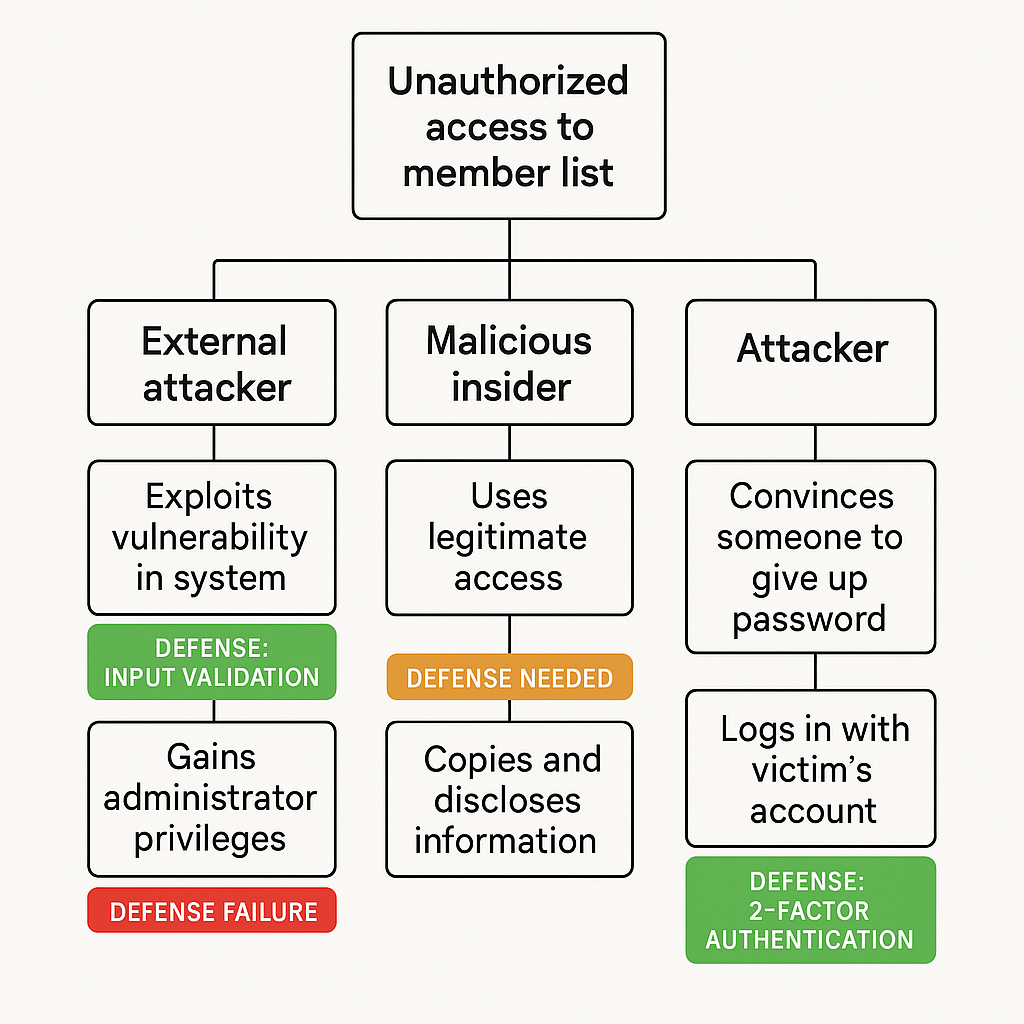
\includegraphics[width=0.6\linewidth]{tree}
        \caption{Attack Tree Example}
        \label{fig:attack_tree_example}
    \end{figure}

    \item \textbf{Conduct Simulations}: Organize simulation exercises for
    more complex scenarios. Assign someone to represent the adversary, while others
    act as defenders or observers. For example, simulate a Sybil attack scenario:
    "Maria secretly created false identities before a vote and uses them to
    influence the results." Go through the steps, discussing whether current
    procedures would detect the attack. This exercise helps reveal weaknesses in a
    safe, low pressure environment rather than during an actual incident.
    This kind of storytelling helps highlight if your current processes have detection or not.

    \item \textbf{Identify Vulnerabilities at Each Step}: For each scenario,
    explicitly identify the weaknesses that make the attack possible including both
    technical issues like outdated software or no data backups and organizational
    issues as no membership verification or one person controls critical knowledge.
    Identify your current controls and assess whether they actually prevent the
    attack or if they can be circumvented. Clearly document these
    vulnerabilities for each scenario, which helps directly inform your mitigation
    efforts.

    \item \textbf{Leverage Past Incidents}: Incorporate experiences from previous
    incidents or near misses to make scenarios more concrete. Ask questions like: Could this
    happen again, perhaps in a more damaging way? or We temporarily lost
    control of our Twitter account before, what if the attackers post harmful content
    next time? Using real world examples helps everyone to understand the severity of
    the threats and the importance of preventive measures.

\end{itemize}

\subsection{Step 6: Prioritize Risks Together}
\label{subsec:Step6}

Which Problems Matter Most?

\subsubsection{Purpose}

This step consists essentially of risk analysis and ranking. Risk is usually judged by two factors:
how severe the impact would be and how likely the threat is to occur. By scoring
or discussing these, the group can focus on the most critical issues.
Importantly, this is done participatorily, everyone's perspective on what is
important is considered, keeping the process democratic. The output will be a
clear list of top risks that the organization will invest effort in mitigating.

\subsubsection{Activities}

\begin{itemize}

    \item \textbf{Define Impact and Likelihood}: First, agree on clear
    definitions for impact and likelihood: high impact risks threaten the
    organization's survival, break laws, or deeply harm member trust; medium impacts
    create noticeable but manageable problems; low impacts result in minor
    inconveniences. High likelihood means there's strong evidence a risk can easily
    happen, medium is conditional, and low likelihood means it's rare or requires
    sophisticated effort.
    
    \item \textbf{Evaluate Each Threat Scenario}: Review your scenarios from Step 3 to 5 one by one,
    asking two questions: If this happens, how bad is it? (Impact) and How likely
    is it? (Likelihood). Different perspectives matter, for example, tech members
    might know a threat is difficult to execute (low likelihood), while governance
    experts could emphasize the severe impact on trust.
    
    \item \textbf{Check Against Goals}: Revisit \hyperref[subsec:Step1]{Step 1's} initial assets and objectives.
    Ensure the prioritized risks align with your core mission and values. If
    important assets lack high ranked threats, double check if something was
    overlooked or truly low risk.

\end{itemize}
    
\subsection{Step 7: Mitigations and Governance Decisions}
\label{subsec:Step7}

How Do We Fix or Prevent Issues?

\subsubsection{Purpose}

For each of the top priority threats, figure out what
security measures to implement and how to approve and enforce them
democratically. This step is where you turn analysis into concrete changes:
technical fixes, new or improved policies, training, etc. It is also where you
make sure that implementing these fixes doesn't accidentally centralize power or
violate cooperative principles.

\subsubsection{Activities}

\begin{itemize}

    \item \textbf{Brainstorm Mitigation Options:} These might include technical solutions (software
    updates, two factor authentication, encryption), workflow improvements
    (clear onboarding/offboarding processes, regular backups, peer reviews
    for critical tasks), training and education (phishing awareness, password
    management sessions), and governance policies (emergency decision protocols,
    member identity verification). Discuss how difficult or costly they are, if
    external resources are required, if they introduce significant workflow
    friction, and if they align with organizational values.
    
    \item \textbf{Assign Responsibilities Clearly:} Define clear responsibilities
    for each mitigation task, distributing them among relevant members or working
    groups. Technical tasks should include tech skilled members paired with others
    for transparency. Assign policy drafting and educational roles to suitable teams
    or individuals.
    
    \item \textbf{Integrate into Governance Documents:} Codify agreed upon
    mitigations and emergency protocols into the organization's official
    documentation. Update handbooks or wikis to institutionalize these practices,
    ensuring new members receive proper orientation.
    
\end{itemize}

\subsection{Participation Tips}
\label{subsec:participation_tips}

Successful threat modeling requires that everyone in the organization feels comfortable
and motivated to contribute. In small groups, completing activities in a single meeting is
effective, fostering unity and avoiding repeat sessions. For larger groups, use
brief questionnaires or small group discussions, consolidating ideas later in
plenary to ensure that everyone can contribute.

It is important that members with technical expertise do not dominate the
conversation. Encourage more reserved participants by asking them directly for
their opinions on specific threats or solutions.

Keep a relaxed and creative environment when role playing scenarios or
developing adversarial personas and document decisions transparently,
explaining the reasons clearly, allowing for future review and improvements.

\section*{}
This chapter has presented the core contribution of this research: a threat
modeling protocol designed from the ground up for horizontal organizations. It
is not merely a set of instructions, but a process rooted in the core principles
of horizontality: transparency, decentralization, and democratic participation.
Through a series of collaborative steps, the protocol guides organizations on a
journey from defining what is most valuable to them, to humanizing their
adversaries through personas, and finally to developing mitigations that are not
just technically sound, but democratically legitimate. It is designed to be a
tangible tool, translating abstract security concepts into an accessible,
collective practice. In essence, the protocol provides a pathway for horizontal
organizations to take ownership of their security in a way that strengthens,
rather than subverts, their fundamental values.